After processing the data, it is now possible to create different experiments for predicting locations. Before starting on the different experiments, we wanted to create a general pattern and flow of the experiments, which will be covered first. Thereafter, the different experiments and their evaluation will be covered.

\section{Experiment Flow}
To start off the process, we wanted to create an overall architecture similar to the one shown in \textbf{\autoref{fig:DataArchitecture}}. The data is being prepared for each individual experiment in the \textit{Data Pipeline} phase before reaching the \textit{Experiments} phase.

\begin{figure}[H]
    \centering
    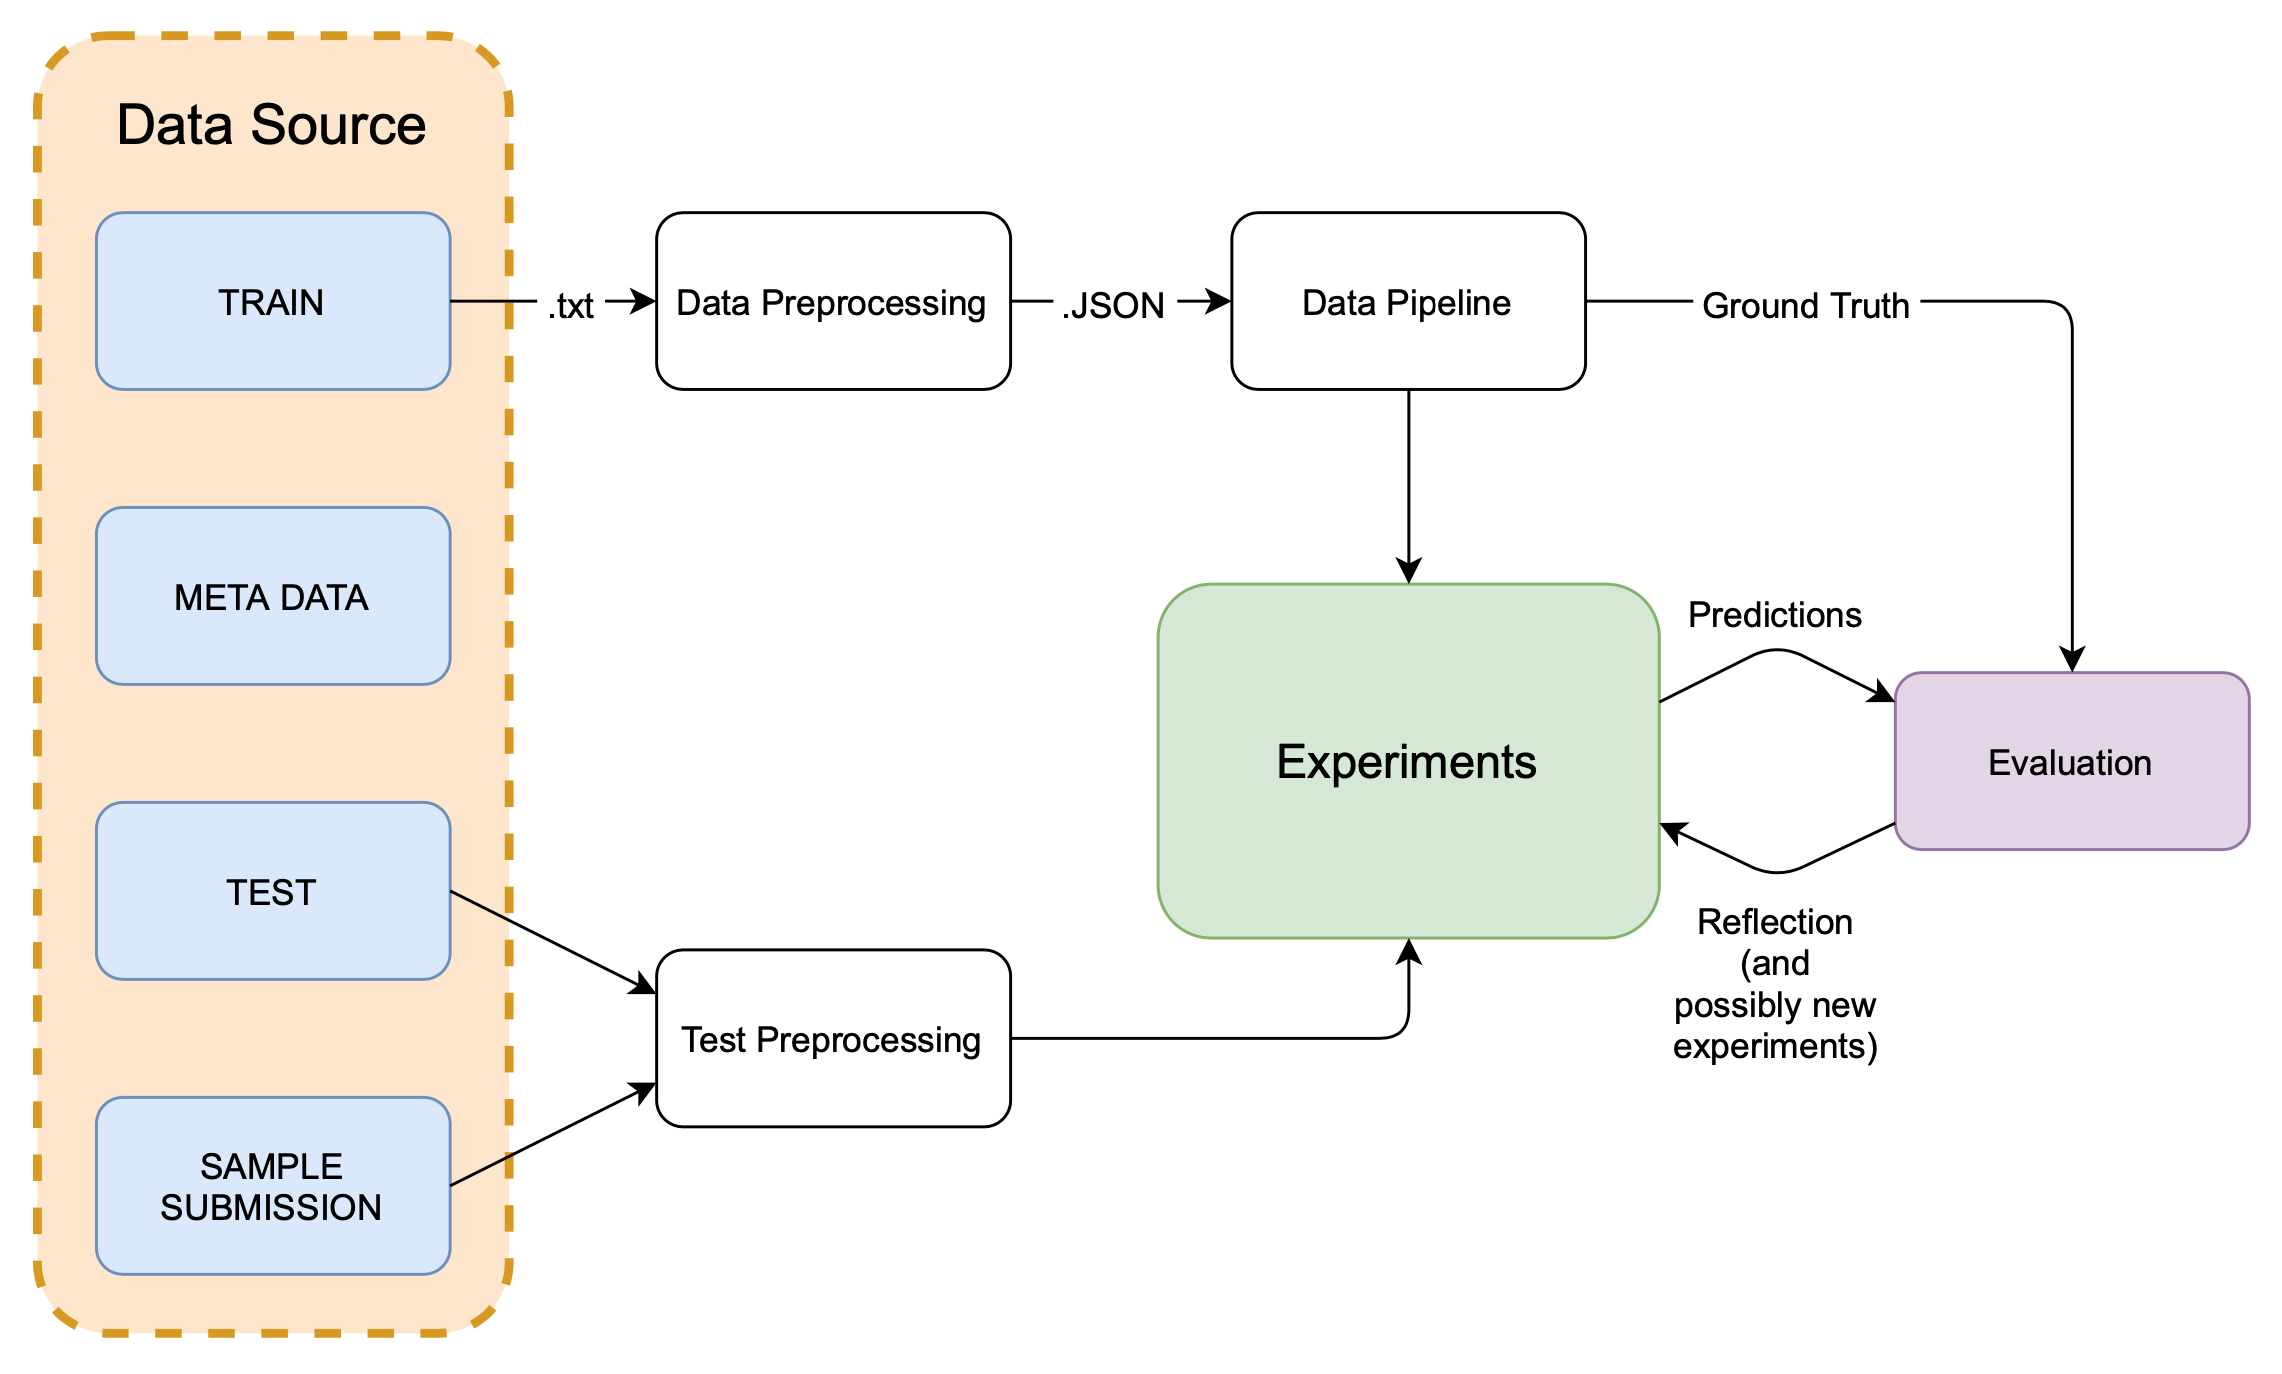
\includegraphics[scale=.34]{Images/Experiments/ExperimentFlow.png}
    \caption{The overall architecture with added evaluation.}
    \label{fig:experimentflow}
\end{figure}

As can be seen on \textbf{\autoref{fig:experimentflow}}, we have expanded on the \textit{Experiments} phase to also interact with the \textit{Evaluation} phase. This new phase takes the ground truth data and compares it to predictions from the experiment. For this purpose, the \textit{Data Pipeline} phase now passes the data to the Experiments phase and also the ground truth data for the \textit{Evaluation} phase. The \textit{Evaluation} phase now compares the result of the experiment to the ground truth and thereby evaluates the experiment. These results can be reflected on, which might lead to new experiments.

\subsection{Experiments}
The \textit{Experiments} phase in \textbf{\autoref{fig:experimentflow}} denotes the implementation and use of the positioning methods, mentioned in \textbf{\autoref{sec:problemstatement}}, which we would need to test. The different experiments will include LightGBM, \gls{ann}, \gls{hmm}, k-NN and \gls{imu}-based methods. Each experiment takes the input data from the \textit{Data Pipeline} phase. As mentioned in \textbf{\autoref{sec:datapipeline}}, this phase is concerned with processing the data for the specific positioning method in the experiment. After receiving the data from the \textit{Data Pipeline} phase, the implementation of the experiment will be executed to achieve estimations of the indoor locations. The estimations from these experiments will then be forwarded to the \textit{Evaluation} phase to determine the performance of the model.
%Elaborate the Experiment part of the design
%Generelt om hvad et eksperiment er + hvilke eksperimenter vi prøver af
%Kontekst til de andre dele (data pipeline + evaluation)
%Input og output til experiments
%

\subsection{K Fold Cross Validation}

\subsection{Evaluation}
To evaluate the different experiments, which is depicted as the \textit{Evaluation} component in \textbf{\autoref{fig:experimentflow}}, we have decided to model a generic Evaluator, which is responsible for the evaluation of the model/algorithm in term of different performance metrics.
%can be used within the experiment to evaluate the performance of the model. 
This Evaluator should evaluate the result with regards to the \gls{mpe} similar to the Kaggle competition mentioned in section \textbf{\autoref{sec:kaggleComp}}. Additionally, it should also calculate the position error with regards to each prediction made by the algorithm/model.

The Evaluator takes the estimations from the \textit{Experiments} phase and the ground truth data from the \textit{Data Pipeline} component as input. From this, it is possible to calculate the position error for each individual estimation. All of the performance metrics as well as the input to the Evaluator should be recorded to a files dedicated for evaluation output. The execution of the generic evaluation class should be integrated into each experiment, where it is possible to work with the results and maybe add additional evaluations.

% NOTER: 
% - Eksperimenter evalueres af single, central evaluator.
% Evaluate waypoints individually with position error
% Evaluator outputter resultater for hver enkelt waypoint.
%   Output indeholder ground truth, estimering, og position error for hvert enkelt prediction.
%   Output konkluderer med mean position error.
% Evaluatator tager ground truth data og estimeringer som input og udregner de nødvendige evalueringer og skriver dem i sidste ende til filer.
% Eksekvering af evaluator skal ske som en integreret del af hvert enkelt eksperiment.
% Evaluator skal generere output i 'output' folder.

%\subsection{Frameworks and Libraries}
%For implementing the different experiments and the generic evaluation class, we have decided to use the programming language Python for consistency with the development of the data handling. We also examined the possibility of implementing all these experiments, where Python seemed like an ideal programming language for this.

%To implement these experiments, we'll be using different frameworks and libraries. For some of the experiments, we have decided to use TensorFlow, which is an open-source machine learning platform.\cite{TensorFlow}
% Vi bruger Python til det hele udover til wrapper til libs.
% Vi bruger det der C++ library (https://github.com/derekblair/DeadReckoner)
% TensorFlow (Neural network, HMM, knn og RNN)
% LightGBM


%\subsection{Coding Standard}
% - Kommentar på alle metoder/funktioner/procedurer.
%   - Kommentarer skal komme den sidste linje før deklaration.
% - Snake-case til symbol deklarationer.
% - 